\documentclass{article}

% if you need to pass options to natbib, use, e.g.:
%     \PassOptionsToPackage{numbers, compress}{natbib}
% before loading neurips_2025

% The authors should use one of these tracks.
% Before accepting by the NeurIPS conference, select one of the options below.
% 0. "default" for submission
% \usepackage{neurips_2025}
% the "default" option is equal to the "main" option, which is used for the Main Track with double-blind reviewing.
% 1. "main" option is used for the Main Track
% \usepackage[main]{neurips_2025}
% 2. "position" option is used for the Position Paper Track
%  \usepackage[position]{neurips_2025}
% 3. "dandb" option is used for the Datasets & Benchmarks Track
% \usepackage[dandb]{neurips_2025}
% 4. "creativeai" option is used for the Creative AI Track
 \usepackage[creativeai]{neurips_2025}
% 5. "sglblindworkshop" option is used for the Workshop with single-blind reviewing
 % \usepackage[sglblindworkshop]{neurips_2025}
% 6. "dblblindworkshop" option is used for the Workshop with double-blind reviewing
%  \usepackage[dblblindworkshop]{neurips_2025}

% After being accepted, the authors should add "final" behind the track to compile a camera-ready version.
% 1. Main Track
% \usepackage[main, final]{neurips_2025}
% 2. Position Paper Track
%  \usepackage[position, final]{neurips_2025}
% 3. Datasets & Benchmarks Track
 % \usepackage[dandb, final]{neurips_2025}
% 4. Creative AI Track
%  \usepackage[creativeai, final]{neurips_2025}
% 5. Workshop with single-blind reviewing
%  \usepackage[sglblindworkshop, final]{neurips_2025}
% 6. Workshop with double-blind reviewing
%  \usepackage[dblblindworkshop, final]{neurips_2025}
% Note. For the workshop paper template, both \title{} and \workshoptitle{} are required, with the former indicating the paper title shown in the title and the latter indicating the workshop title displayed in the footnote.
% For workshops (5., 6.), the authors should add the name of the workshop, "\workshoptitle" command is used to set the workshop title.
% \workshoptitle{WORKSHOP TITLE}

% "preprint" option is used for arXiv or other preprint submissions
% \usepackage[preprint]{neurips_2025}

% to avoid loading the natbib package, add option nonatbib:
%\usepackage[nonatbib]{neurips_2025}
\usepackage[utf8]{inputenc} % allow utf-8 input
\usepackage[T1]{fontenc}    % use 8-bit T1 fonts
\usepackage{hyperref}       % hyperlinks
\usepackage{url}            % simple URL typesetting
\usepackage{booktabs}       % professional-quality tables
\usepackage{amsfonts}       % blackboard math symbols
\usepackage{nicefrac}       % compact symbols for 1/2, etc.
\usepackage{microtype}      % microtypography
\usepackage{xcolor}         % colors
\usepackage{tikz}           % diagrams
\usepackage{enumitem}       % customized lists
\usepackage{natbib}
\usetikzlibrary{arrows.meta,shapes,positioning,fit,backgrounds,calc}

% Note. For the workshop paper template, both \title{} and \workshoptitle{} are required, with the former indicating the paper title shown in the title and the latter indicating the workshop title displayed in the footnote. 
\title{Simulated Profiling Environment for Embodied I\underline{n}telligence (SPEEN)}


% The \author macro works with any number of authors. There are two commands
% used to separate the names and addresses of multiple authors: \And and \AND.
%
% Using \And between authors leaves it to LaTeX to determine where to break the
% lines. Using \AND forces a line break at that point. So, if LaTeX puts 3 of 4
% authors names on the first line, and the last on the second line, try using
% \AND instead of \And before the third author name.

\author{%
    Darroll Saddi\textsuperscript{1} \quad
        Ken Lin\textsuperscript{1} \quad
        Ryan Li\textsuperscript{1} \quad
        Matthew Fulde\textsuperscript{2} \quad
        Jon Lagasca\textsuperscript{1} \vspace{0.75em} \\
        \large{\textit{University of California, Davis}} \\
        \vspace{0.5em}
        \textsuperscript{1}Computer Science \quad
        \textsuperscript{2}Computer Science and Engineering \\
        \texttt{\{dwsaddi, kemlin, ryjli, mpfulde, jonlagasca\}@ucdavis.edu}
    }

\begin{document}

\maketitle

\begin{abstract}
    The Simulated Profiling Environment for Embodied Intelligence (SPEEN) is an open-source platform for evaluating embodied Large Language Model agents in a simulated game environment.
    As LLMs are increasingly integrated into robotics and embodied systems, SPEEN addresses the critical need for standardized evaluation frameworks by providing a modifiable system for benchmarking and implementing embodied LLM simulations in Godot.
    We implement a proof-of-concept Minecraft-like environment to demonstrate an application of this system, providing both structured quantitative benchmarking through diverse scenarios and an open-world sandbox for qualitative assessment of decision-making behaviors.
    Our system provides researchers a tool to test various embodied LLM implementations in a flexible simulated environment and contribute to the development of robust evaluative measures for Trustworthy AI.
    \begin{figure}[ht!]
        \centering
        \begin{minipage}[b]{0.47\textwidth}
            \centering
            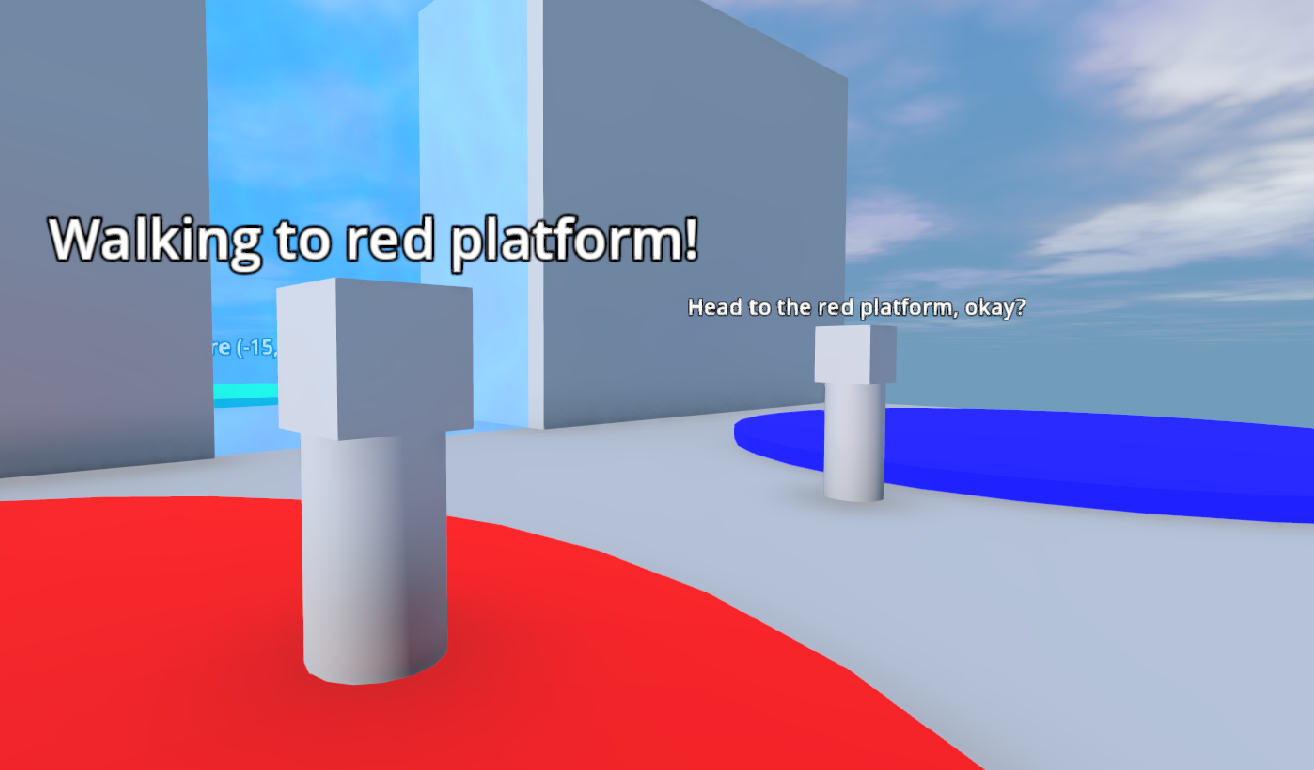
\includegraphics[width=\textwidth]{./example.png}
        \end{minipage}
        \hfill
        \begin{minipage}[b]{0.47\textwidth}
            \centering
            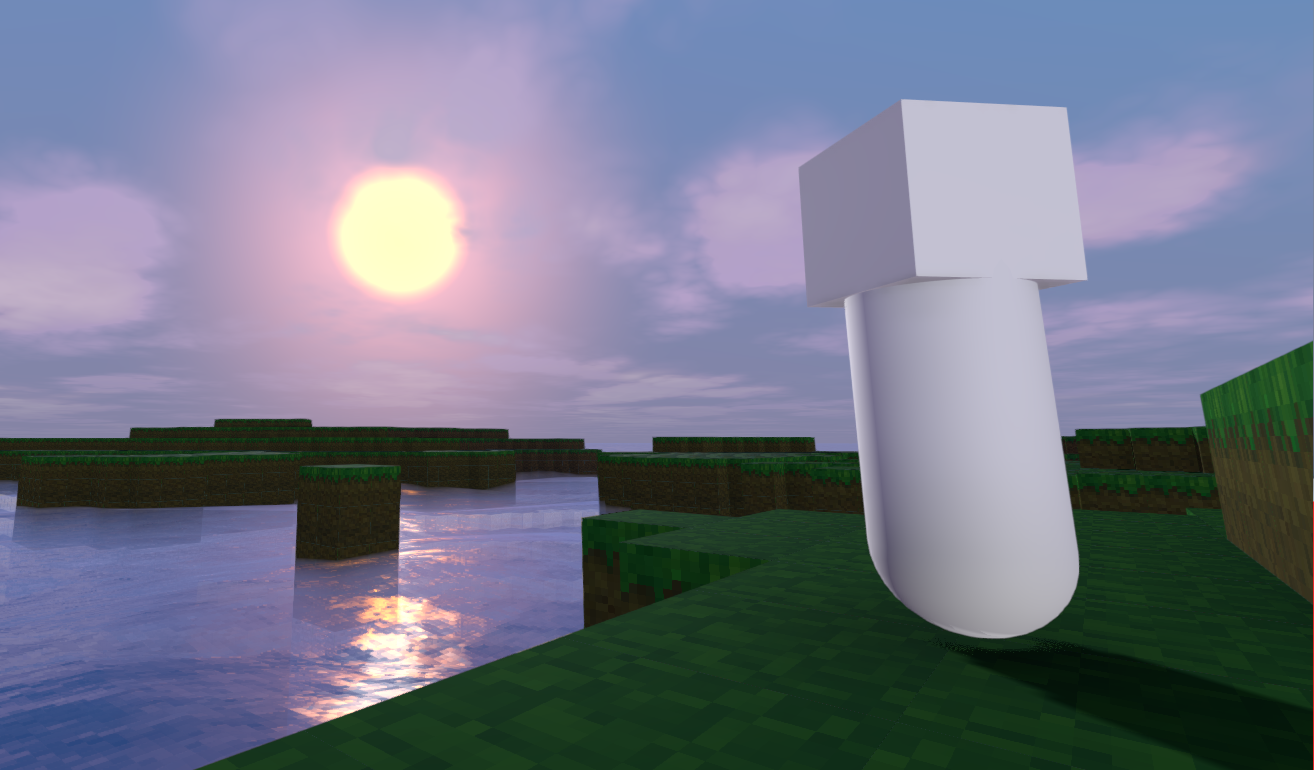
\includegraphics[width=\textwidth]{./example2.png}
        \end{minipage}
        \caption{SPEEN simulation environment screenshots}
        \label{fig:speen-environment}
    \end{figure}
\end{abstract}

\section{Problem Identification}

\paragraph{Background}
This project originated as a Senior Design Project at UC Davis in collaboration with Justin Jia (affiliated with Apple) to address practical needs in AI testing.
The overarching goal of the project at this stage was to develop a sandbox environment specifically for testing AI programs.

\subsection{Exploratory Research}

\paragraph{Definitions}
We define agentic AI as systems capable of autonomous decision-making and environmental interaction, with embodied AI specifically concerning agents that interact with physical or simulated worlds.

\subsubsection{Focusing on Large Language Models}
Our research identified significant gaps in environmental design for evaluating advanced AI systems.
We examined existing platforms like NeuralMMO, which provides an open-source environment for measuring \textbf{reinforcement learning} algorithm performance.
It does this by implementing a 2D grid world with a variety of complex tasks that emulate a massively multiplayer online game.
A key insight from NeuralMMO's creator Joseph Suarez influenced our approach:
\begin{quote}
    "It is very easy to create an interesting looking simulator. It is very hard, under the constraints of making useful AI research [to create an environment meant for testing and training AI]…it is not just a game, it is an AI simulation."\footnote{Suarez, J. (2024, May 14). Joseph Suarez Thesis Defense - Neural MMO. YouTube. \url{https://www.youtube.com/watch?v=wwTOFYgtAWg}.}
\end{quote}
Furthermore, despite increasing environmental complexity, advanced algorithms like PPO were observed to be able to effectively solve most tasks given sufficient computation.
This shifted our focus toward Large Language Models, which have shown recent promise in integration with robotics and embodied systems.

\subsubsection{Environment Design}
There are a number of proposed embodied LLM architectures that use Minecraft as a testing environment.
Projects including NVIDIA's Voyager project (extending from the MineDojo project) and Project Sid by Altera\footnote{AL, A., Ahn, A., Becker, N., Carroll, S., Christie, N., Cortes, M., Demirci, A., Du, M., Li, F., Luo, S., Wang, P. Y., Willows, M., Yang, F., \& Yang, G. R. (2024). Project Sid: Many-agent simulations toward AI civilization. \url{https://arxiv.org/abs/2411.00114}.} attempt to provide prompting and training architectures for agents to exist in the game.
However, these projects exhibit several critical limitations as benchmarks for agentic LLMs:
\begin{itemize}[noitemsep,topsep=0pt]
    \item \textbf{Lack of Open-Source Availability:}
          Project Sid articulates a way for many-agents to exist within Minecraft, proposing supposedly powerful prompting architectures.
          However, it is not open-source.
          This means their methodology for reproducing their results is not easily reproducible, potentially creating barriers to validation and further scientific progress.
    \item \textbf{Limited Flexibility:}
          While MiniDojo projects like NVIDIA's Voyager\footnote{Wang, G., Xie, Y., Jiang, Y., Mandlekar, A., Xiao, C., Zhu, Y., Fan, L., \& Anandkumar, A. (2023). Voyager: An Open-Ended Embodied Agent with Large Language Models. \url{https://doi.org/10.48550/arXiv.2305.16291}.} have yielded impressive results and are open-source, we believe there is an increasing need to develop benchmarks that generalize to real-world use cases.
          Additionally, metrics that evaluate agentic LLMs more generally, as opposed to domain-specific ones like 'area explored' or 'percentage of items collected', would also help expand to real-world applications of the technology.
\end{itemize}

\vspace{-0.5em}
Additional barriers exist in the choice of environment.
While Minecraft offers inherent complexity and extensive documentation as an additional input to AI training, it presents significant limitations as a benchmark:
\begin{enumerate}[noitemsep]
    \item It requires a commercial license, creating accessibility barriers
    \item There are no existing standardized context provisioning or testing metrics
\end{enumerate}

\paragraph{Chosen Environment} While environments that closely emulate the real world would map better to real-world robotic applications, we believed that focusing on standardizing an accessible contextualization and prompting system would make our project more beneficial for future work.
Thus, our primary goal was to develop a modifiable prompting architecture---i.e., the interaction between the LLM and the game environment---and the evaluation of agentic LLMs in an equally modular simulated environment.
With this in mind, we designed our environment to be relatively simple for our proof-of-concept, but we hope that future work will expand our systems to more realistic or complex environments.

\subsubsection{Open-Source}
To address the limitations of inaccessible LLM projects, which limit their utility for broader research purposes, we built our system to allow for transparent and reproducible integrations of new LLMs and prompting architecture, in addition to being used as a benchmark.
These goals guided our decision to use the Godot game engine, which is open-source and allows for easy modification and expansion, and allows us to export the game environment in a packaged format.
Our selection of Godot was also motivated by its rapid development trajectory and growing community support, with major improvements in each release enhancing both performance and development workflows, showing great promise for use beyond simply game development.

\subsubsection{Research Use Case}
Ensuring our backend Python websocket supports both cloud-hosted and locally-hosted LLMs is important for allowing researchers to test various models as they're released.
Using abstraction layers, new models can be integrated into the system without requiring significant changes to the code base on the development side.
We implemented several different scenarios that stress test our API and agents capabilities for planning, environmental reasoning, and cooperation.
In the current product, we support the OpenAI GPT models, Google Gemini API, locally-hosted LLMs via OLlamma (Gemma3, Deepseek-r1, etc.).

\subsection{Design Requirements}
Based on our research findings, we had sufficient justification to develop SPEEN as an open-source benchmarking environment for evaluating embodied AI (LLM) performance.
Listed below are our comprehensive design goals and requirements for the system:
\begin{enumerate}[noitemsep,topsep=0pt]
    \item \textbf{Standardized Evaluation Framework:}
          \begin{itemize}[noitemsep,topsep=0pt]
              \item Quantitative metrics and qualitative assessment for embodied LLM agents
              \item Standardized prompting and game state context provisioning
              \item Streamlined integration of LLMs, prompting architectures, and evaluation methods
          \end{itemize}
    \item \textbf{LLM Integration Capabilities:}
          \begin{itemize}[noitemsep,topsep=0pt]
              \item Support for cloud and locally-hosted LLMs
              \item Abstraction layers for seamless integration of any LLM
              \item High-level configuration options
          \end{itemize}
    \item \textbf{Open-Source Compliance:}
          \begin{itemize}[noitemsep,topsep=0pt]
              \item Accessible and modifiable system with appropriate licensing for research purposes
              \item Comprehensive documentation
          \end{itemize}
\end{enumerate}
\vspace{-0.5em}
To prove its usability, we shall also implement the testing environment and prompting architecture as a proof of concept.
\begin{enumerate}[noitemsep]
    \item \textbf{Accessible Game Environment:} A Minecraft-like 3D environment in Godot with sufficient complexity and intuitive interfaces for human researchers to monitor and evaluate agent performance
    \item \textbf{Structured Scenarios:} Diverse testing scenarios with automated performance scoring
    \item \textbf{Prompting Architecture:} Implemented a prompting architecture emulating chain-of-thought and goal-based prompting systems with support for easy modification
\end{enumerate}

\subsection{Agent-Environment Pipeline}
\begin{figure}
    \centering
    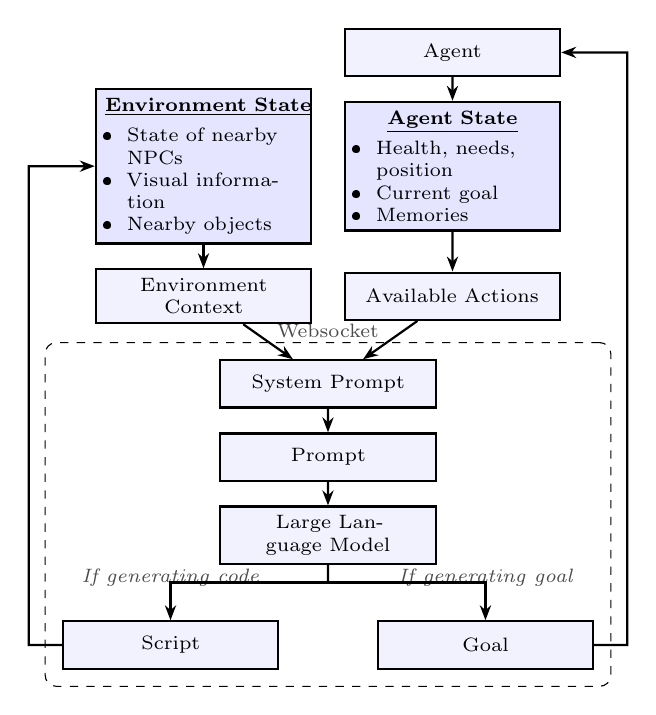
\begin{tikzpicture} [
        scale=0.15,
        node distance=0.4cm,
        box/.style={
                rectangle,
                draw,
                thick,
                minimum width=2cm,
                minimum height=1.5cm,
                text width=2.5cm,
                align=center,
                fill=blue!10,
                font=\scriptsize,
            },
        smallbox/.style={
                rectangle,
                draw,
                thick,
                minimum width=2cm,
                minimum height=0.6cm,
                text width=2.5cm,
                align=center,
                fill=blue!5,
                font=\scriptsize,
            },
        arrow/.style={-{Stealth[length=1.9mm]}, thick},
        condition/.style={font=\scriptsize\itshape, text opacity=0.7},
        ]
        % Define main component layer
        \node[box] (env) {\textbf{\underline{Environment State}} \\
            \begin{itemize}[leftmargin=1em, itemsep=0pt, topsep=1pt, parsep=0pt]
                \item State of nearby NPCs
                \item Visual information
                \item Nearby objects
            \end{itemize}};

        \node[box, right=of env] (agent_state) {\textbf{\underline{Agent State}} \\
            \begin{itemize}[leftmargin=1em, itemsep=0pt, topsep=1pt, parsep=0pt]
                \item Health, needs, position
                \item Current goal
                \item Memories
            \end{itemize}};

        \node[smallbox, above=0.3cm of agent_state] (agent) {Agent};

        % Context processing layer - all on the same layer
        \node[smallbox, below=0.3cm of env] (env_context) {Environment Context};
        \node[smallbox, right=of env_context] (actions) {Available Actions};

        % Calculate midpoint position for system prompt - now below env_context and actions
        \path (env_context) -- (actions) coordinate[midway] (mid_point);
        \node[smallbox, below=0.8cm of mid_point] (system_prompt) {System Prompt};

        % Prompt layer - moved down
        \node[smallbox, below=0.3cm of system_prompt] (prompt) {Prompt};

        % Connect system prompt to prompt
        \draw[arrow] (system_prompt) -- (prompt);

        % LLM layer - moved down
        \node[smallbox, below=0.3cm of prompt] (llm) {Large Language Model};

        % Output layer - centered below LLM with appropriate spacing
        \path (llm.south west) -- (llm.south east) coordinate[midway] (llm_bottom);
        \node[smallbox, below=0.7cm of llm, xshift=-2cm] (script) {Script};
        \node[smallbox, below=0.7cm of llm, xshift=2cm] (goal) {Goal};

        % Add websocket label
        \node[draw, dashed, rounded corners, fit=(prompt)(system_prompt)(llm)(script)(goal), inner sep=6pt] (websocket_box) {};  % Reduced inner sep from 8pt to 6pt
        \node[font=\scriptsize, text opacity=0.7, yshift=4pt] at (websocket_box.north) {Websocket};

        % Main connections
        \draw[arrow] (env) -- (env_context);
        \draw[arrow] (agent_state) -- (actions);
        \draw[arrow] (agent) -- (agent_state);
        \draw[arrow] (env_context) -- (system_prompt);
        \draw[arrow] (actions) -- (system_prompt);
        \draw[arrow] (prompt) -- (llm);

        \draw[thick] (llm) -- ++(0,-4) coordinate (branch_point);
        \draw[arrow] (branch_point) -| (script);
        \draw[arrow] (branch_point) -| (goal);

        \node[condition, below=-0.075cm of llm, xshift=-2cm] {If generating code};
        \node[condition, below=-0.075cm of llm, xshift=2cm] {If generating goal};

        \draw[arrow] (script) -- ++(-12,0) |- (env.west);
        \draw[arrow] (goal) -- ++(12,0) |- (agent.east);
    \end{tikzpicture}
    \caption{Agent-Environment Pipeline Architecture}
    \label{fig:agent-pipeline}
\end{figure}

\section{Development}
\subsection{Environment Design}
The majority of early development focused on creating the agent's environment for qualitative evaluation.
Features included procedural world generation with day/night cycle, navigation and A* pathfinding via Godot's Navigation3D system, a suite of API functions for agent-environment interaction, NPC AI (animals, zombies) for objectives and adversaries, and an item and inventory system.
After 7 weeks, we had a functional environment sufficiently complex for our proof of concept.

Figure \ref{fig:agent-pipeline} illustrates our agent-environment pipeline architecture, which also serves as our prompting architecture.
Environmental information is fed directly into the LLM, which either generates a script containing the desired actions based on the current goal, or generates a new goal after completing a previous task.
The generated script is executed by the environment, and the outcome is logged in the agent's "Memories," which updates the agent state, enabling persistent contextual awareness across iterations. This memory system implements chain-of-thought reasoning, allowing the agent to build upon previous experiences and maintain contextual awareness across multiple decision cycles, which proved crucial for solving complex sequential tasks.

The available actions are provided in the System Prompt, designed to remove the need for low-level implementation details and allow the benchmark to focus on reasoning and decision-making.
For error handling, we implemented a system that catches broken code and can either re-prompt the LLM with the specific error for self-correction, or count the iteration as a failure for benchmarking.
Once validated, the agent's "body" executes the actions sequentially until completion. 
The pipeline then repeats, gathering updated environmental information and continuing until either the scenario goal is satisfied or the maximum allowed iterations is reached.

\section{Testing and Evaluation}
\subsection{Quantitative Testing}
We implemented several types of scenarios to test different aspects of agent capabilities:
\textbf{(1) Prompt adherence scenarios} test navigation and item manipulation to evaluate the agent's ability to correctly control their virtual body;
\textbf{(2) Entity interaction scenarios} assess the agent's ability to react to and interact with changes in real-time entity state;
\textbf{(3) Sequential reasoning tasks} evaluate the agent's ability to perform multi-step tasks requiring planning; and
\textbf{(4) Multi-agent tasks} test many-agent interaction in scenarios requiring collaboration or competition.

Our benchmarking toolkit automatically tracks performance metrics including success rate, completion time, and error recovery attempts for each scenario. 
We designed the system to detect and categorize failures, including code compilation errors that can potentially be repaired, and timeouts where the agent fails to make progress within a reasonable timeframe.
Figure \ref{tab:model-performance} shows the performance of three different LLMs in our testing scenarios.

\subsection{Qualitative Testing}
Beyond quantitative metrics, we conducted qualitative evaluations to assess agent behavior in open-ended scenarios. Our observations revealed several notable patterns:
Our environment and prompting architecture designs translated well to the following qualitative observations, which we believe are important for future work in embodied AI:
\paragraph{Chain of Thought} When allowed to iteratively set goals and react to the results of their own actions, agents were able to succeed in more complex tasks.
\paragraph{Adaptability} By providing standardized context, a basic system prompt, both supported by the memory system, we observed that most LLMs were capable of adapting to available information within the environment and performing the task effectively.
For multimodal LLMs capable of vision, the additional visual information proved advantageous as this additional context helped influence its decision-making.
In implementation, our system designs enabled easy integration of the environment, prompting architecture, and LLMs.

\paragraph{Cooperative Behavior} In multi-agent scenarios, we observed emergent cooperative behaviors which would develop division-of-labor strategies without explicit prompting.
This emergent coordination suggests potential for more complex social dynamics in future iterations of the system.
Further evaluative research into the effectiveness of deployments of these types of systems in real-world applications is also promising.
\begin{figure}
    \centering
    \small
    \begin{tabular}{lccc}
        \toprule
        \textbf{Scenario Type} & \textbf{GPT-4} & \textbf{Claude 3} & \textbf{Gemini Pro} \\
        \midrule
        \multicolumn{4}{l}{\textit{Success Rate (\%)}} \\
        Prompt adherence        & 92 & 88 & 84 \\
        Entity interaction      & 85 & 80 & 75 \\
        Sequential reasoning    & 76 & 72 & 65 \\
        Multi-agent             & 70 & 65 & 58 \\
        \midrule
        \textbf{Overall Success} & \textbf{81} & \textbf{76} & \textbf{71} \\
        \bottomrule
    \end{tabular}
    \caption{Performance comparison of different LLM models across test scenarios \answerTODO{remove placeholders}} 
    \label{tab:model-performance}
\end{figure}

\section{Significance}
\subsection{Trustworthy AI}
As embodied AI systems become increasingly integrated into real-world applications, establishing trust through rigorous evaluation becomes paramount.
SPEEN directly addresses this need by providing a simulation framework for testing and benchmarking LLMs in a controlled setting, allowing researchers and developers to assess the reliability and safety of their agentic \& embodied AI systems and architectures before deployment.
Our current product accomplishes this by providing the following: 

\textbf{(1) Reproducible Benchmarking:} Our open-source and easily modifiable environment allows for the extension of our system to new scenarios and architectures, enabling reproducible testing across different models and implementations.
This establishes a foundation for valid comparisons and trustworthy claims about model capabilities.

\textbf{(2) Simulated Testing:} By allowing researchers to test different prompting architectures and LLMs in a controlled environment, SPEEN enables evaluation of prompting strategies, LLM performance, agent behavior, and overall effectiveness of embodied AI systems before real-world deployment.

\textbf{(3) Standardized Metrics:} SPEEN provides consistent scenarios that evaluate embodied AI systems across multiple dimensions, including planning, reasoning, task completion, adaptability, and cooperation, facilitating meaningful comparisons between different approaches.

\subsection{Transitioning AI Research Into Production}
SPEEN bridges the gap between research and application of new AI technologies by introducing a standardized evaluation framework for the emerging field of embodied AI.
We believe it is critical that AI systems undergo rigorous testing and evaluation before deployment, and SPEEN provides a platform for researchers to assess the performance and reliability of their models in a controlled environment.
As previously mentioned, we believe that allowing our systems to be extended to new architectures and models is critical to the success of our project as a benchmarking and testing framework.
We therefore place an emphasis on the clean documentation of our system and the extensibility of the different components that make up SPEEN, always keeping in mind the potential for our work to be further developed.
By providing these capabilities, SPEEN contributes to the responsible advancement of embodied AI from research concepts to practical applications, helping ensure that both our current systems and future systems are able to be used reliably, safely, and effectively.

\section{Conclusion and Future Work}
Large Language Models are a relatively new technology, with limited tools available for measuring their competency in decision-making and environment interaction, particularly in embodied contexts. While existing projects such as Mindcraft\footnote{kolbytn. (2023). GitHub - kolbytn/mindcraft. GitHub. \url{https://github.com/kolbytn/mindcraft}.} and Voyager integrate LLMs into virtual worlds, they lack comprehensive benchmarking features and require commercial licenses, creating barriers to research accessibility.

SPEEN addresses these limitations by providing an open-source, flexible framework for rigorous evaluation of embodied LLM agents.
Our system's design allows for seamless integration of different LLMs, coupled with standardized benchmarking scenarios designed to be easily modifiable, offering researchers a valuable tool for comparative analysis of embodied AI systems.

Future work could focus on three key areas: (1) expanding the range of testing scenarios to cover more diverse and challenging tasks, (2) developing more sophisticated multi-agent interactions to assess emergent social behaviors, and (3) refining evaluation metrics to better correlate with real-world application requirements.
Further development may also include better approximating real-world environments of embodied AI systems in robotics and beyond.

By making SPEEN available to the broader research community, we hope to accelerate progress in embodied AI by establishing common standards for evaluation and comparison, ultimately contributing to the development of more capable, reliable, and trustworthy embodied intelligence systems.

\end{document}